\documentclass[10pt,prd,aps,a4paper,twocolumn,superscriptaddress,nofootinbib,floatfix]{revtex4-2}
\pdfoutput=1

\usepackage[T1]{fontenc}
\usepackage[utf8]{inputenc}
\usepackage{lmodern}

\usepackage{amsmath,amssymb,amsfonts,bm,mathrsfs}

\usepackage{graphicx}
\usepackage{booktabs}
\usepackage{dcolumn}

\usepackage{color}

\makeatletter
\newcommand{\adddotsbeforeeqnnum}{%
    \renewcommand{\theequation}{\arabic{equation}.}%
}
\makeatother

\usepackage{braket}

\usepackage[linktoc=none]{hyperref}
\hypersetup{colorlinks,			
	linkcolor=blue,
	citecolor=blue}

\begin{document}

\title{Reconstruction of Black Hole Ringdown Signals with Data Gaps using a Deep-Learning Framework}
\author{Jing-Qi Lai}\email{laijingqi19@mails.ucas.ac.cn}
\affiliation{School of Physical Sciences, University of Chinese Academy of Sciences, Beijing 100049, China}
\author{Jia-Geng Jiao}\email{jiaojiageng@ucas.ac.cn}
\affiliation{International Centre for Theoretical Physics Asia-Pacific,
University of Chinese Academy of Sciences, Beijing 100190, China
}
\author{Cai-Ying Shao}\email{shaocaiying@ucas.ac.cn}
\affiliation{School of Physical Sciences, University of Chinese Academy of Sciences, Beijing 100049, China}

\author{Jun-Xi Shi}\email{shijunxi23@mails.ucas.ac.cn}
\affiliation{International Centre for Theoretical Physics Asia-Pacific,
University of Chinese Academy of Sciences, Beijing 100190, China
}
\author{Yu Tian}\email{ytian@ucas.ac.cn}
\affiliation{School of Physical Sciences, University of Chinese Academy of Sciences, Beijing 100049, China}
\affiliation{Institute of Theoretical Physics, Chinese Academy of Sciences, Beijing 100190, China}

\begin{abstract}
Data gaps near the onset of black hole ringdown can obscure much of its rapidly decaying signal. We present DenoiseGapFiller (DGF), a neural network that jointly denoises and reconstructs ringdown waveforms using complementary time--frequency and temporal representations. We evaluate DGF on 6,000 independent simulated LISA observations with gaps spanning approximately 6\%--10\% of each record. For network signal-to-noise ratios $\rho\ge10$, the mean direct noise-weighted mismatch is $5.32\times10^{-3}$ at fixed arrival time and phase. The corresponding mean over all 6,000 test signals is $8.52\times10^{-3}$. Across the full test population, the mean absolute analytic-phase error at each channel's clean-signal envelope peak is below $4^\circ$. These results demonstrate recovery of the oscillatory waveform across gaps, including intervals containing the signal peak, within the simulated source population and stationary Gaussian instrument-noise model.
\end{abstract}

\maketitle
\section{Introduction}
The ringdown following a binary black hole merger carries information about the remnant spacetime. In the perturbative regime, its waveform is described by damped quasinormal modes whose frequencies and decay times depend on the mass and spin of a Kerr black hole~\cite{berti2006gravitational,berti2009qnm}. Measuring these modes is the basis of black hole spectroscopy and ringdown tests of general relativity~\cite{Isi_2019}. Space-based observatories such as LISA, Taiji and TianQin offer access to the ringdowns of massive black hole binaries in the millihertz band~\cite{amaroseoane2017laserinterferometerspaceantenna,robson2019construction,Ruan2020,Luo2016}.

Ringdown amplitudes decay rapidly. An interruption near the onset can therefore remove a substantial fraction of the signal even when its duration is short compared with the analysis window. Scheduled interruptions and unscheduled data losses are relevant to space-based observations~\cite{Baghi2019,dey2021gaps}. Shi \textit{et al.}~\cite{shi2024effectsdatagapsringdown} examined their effects on ringdown observability and parameter estimation. Multiplication by a gap window also redistributes power across Fourier frequencies~\cite{Harris1978}. We study 32--52-s gaps in 528-s records, corresponding to approximately 6\%--10\% of the analysis window, and assess waveform overlap, amplitude error and phase recovery across the gap.

Existing approaches exploit different information about the missing signal. Interpolation uses neighboring samples, with accuracy determined by the bandwidth, sampling and interpolation rule~\cite{Horowitz1974,Maeland1988,Unser1999}. Bayesian data augmentation treats missing samples as latent variables in source-parameter inference~\cite{Baghi2019}. Sparse representations provide a basis for inpainting~\cite{Starck2010}; Fourier sparsity has been used to recover Galactic-binary signals in gapped LISA data~\cite{Blelly2021}. Learned dictionaries provide another way to encode waveform structure for denoising~\cite{TorresForne2016}. Ringdown reconstruction poses a specific challenge for these approaches: the waveform is oscillatory, its envelope changes rapidly, and the available context can be strongly asymmetric about the gap.

Neural methods learn reconstruction maps from simulated waveforms and noisy observations. Xu \textit{et al.}~\cite{Xu_2024} used a DenseNet--BiLSTM model for inspiral--merger--ringdown signals under several forms of corruption. Mao \textit{et al.}~\cite{Mao:2025cae} combined a convolutional autoencoder with a bidirectional gated recurrent unit for long LISA sequences containing gaps. WaveFormer~\cite{Wang:2024waveformer} combines convolutional feature extraction and Transformer blocks for denoising ground-based data, and assesses amplitude and phase recovery separately. Here we focus on short ringdown records, where a gap can cover the amplitude peak and leave substantially different signal strengths on its two sides.

We develop DGF to recover damped oscillations from noisy observations with a known gap. The time--frequency branch represents local oscillatory content through complex Morlet continuous wavelet transform (CWT) coefficients. The temporal branch preserves the sign and multiscale structure of the waveform. Mixing layers combine these complementary features, and sequence blocks connect context on both sides of the interval before a decoder synthesizes the clean waveform. Related time-series models use temporal and feature mixing to combine information across scales~\cite{TSMixer2023,TimeMixer2024}. Whitening uses a calibrated power spectral density (PSD), while mask-aware and joint-channel modules refine the decoded waveform. A coefficient head adjusts the coefficients of a fixed, training-derived signal basis using observation-derived noise and phase features.

The observation model is $d=Gh+n$: $G$ suppresses the signal over one interval, and noise is present throughout the record. We report reconstruction accuracy for $\rho\ge10$ alongside the complete test population, and examine recovery across intervals containing the signal-envelope peak.

Section~\ref{sec:method} presents the reconstruction framework, signal and noise models, and training protocol. Section~\ref{sec:results} evaluates waveform recovery, gap-location dependence, amplitude fidelity and phase accuracy. Section~\ref{sec:discussion} discusses the implications for ringdown analysis and the scope of the simulations. The appendixes give implementation and reproducibility details, fixed-duration gap tests and a comparison with a reference DGF configuration.

\section{Methodology}\label{sec:method}
We generate simulated ringdown observations using standard LISA response and noise models. DGF operates on the $A/E$ time-delay interferometry (TDI) channels and estimates their complete clean waveforms from the observations and known gap mask. The signal, response, noise calibration and preprocessing described below are shared by the training, validation and independent test sets.

\subsection{Physical ringdown signals and LISA response}\label{sec:physical_signals}
The source population consists of nonspinning progenitor binaries. The source-frame total mass $M_{\rm tot}^{\rm src}$ is drawn log-uniformly from $10^5$ to $5\times10^6\,M_\odot$, the light-to-heavy mass ratio $q=m_2/m_1$ uniformly from $0.3$ to $1$, and redshift $z$ uniformly from $1$ to $6$. Sky position and inclination are isotropic; polarization and orbital phase are uniform on their angular ranges. We use a flat $\Lambda$CDM distance relation with $H_0=67.4\,\mathrm{km\,s^{-1}\,Mpc^{-1}}$ and $\Omega_m=0.315$.

The SEOBNRv4 remnant prescription in LALSuite 7.25.1 determines the source-frame remnant mass $M_f^{\rm src}$ and dimensionless spin $\chi_f$. The Kerr-mode frequencies and damping times use the detector-frame remnant mass,
\begin{equation}
M_f^{\rm det}=(1+z)M_f^{\rm src}.
\end{equation}
The fundamental modes $(\ell,m,n)=(2,2,0),(2,1,0),(3,3,0),(4,4,0)$ enter the PyCBC time-domain ringdown generator~\cite{berti2006gravitational,berti2009qnm,PyCBCRingdown}. We use spin-weight $-2$ spherical harmonics in the PyCBC convention. The dimensionless strain amplitudes include the mass--distance factor $G_{\rm N}M_f^{\rm det}/(c^2D_L)$, where $G_{\rm N}$ is Newton's constant and $D_L$ the luminosity distance. The complex polarization $h_++ih_\times$ is passed to the response calculation. Writing $q_\star=1/q$, the mode excitation coefficients are~\cite{Kamaretsos2012}
\begin{align}
\alpha_{22}&=0.25e^{-q_\star/7.5},\nonumber\\
\frac{\alpha_{21}}{\alpha_{22}}&=0.13(q_\star-1)^{1/2},\qquad
\frac{\alpha_{33}}{\alpha_{22}}=0.18(q_\star-1)^{1/3},\nonumber\\
\frac{\alpha_{44}}{\alpha_{22}}&=0.024q_\star^{3/4}.
\end{align}
These fits refer to the reference epoch used by Kamaretsos \textit{et al.}, ten remnant-mass time units after the dominant-mode luminosity peak. The relative phase convention is $\phi_{\ell m}=m\phi_{\rm orb}$. It defines a simplified coherent mode family for this reconstruction study. For a mode with damping time $\tau_{\ell m}$, the pre-reference amplitude varies as $e^{10t/\tau_{\ell m}}$ for $t_s\le t<0$ and as $e^{-t/\tau_{\ell m}}$ for $t\ge0$. PyCBC sets the common start to $t_s=-\lceil\tau_{\max}/\Delta t\rceil\Delta t$, with $\tau_{\max}$ the longest included damping time; the earlier strain is zero. The oscillatory phase evolves continuously through $t=0$, and both envelope branches have the same amplitude there. The one-sided envelope slopes differ. This prescribed history enters the TDI delays and is included in the reconstruction targets.

The polarizations are projected onto the constellation links with \texttt{fastlisaresponse}~\cite{Katz2022Response}. Delayed link combinations produce second-generation TDI $X,Y,Z$ observables in an idealized equal-arm constellation. The analyzed channels are
\begin{equation}
A=\frac{Z-X}{\sqrt{2}},\qquad E=\frac{X-2Y+Z}{\sqrt{6}}.\label{eq:aet_convention}
\end{equation}
Both channels are expressed in fractional-frequency units. We generate the response on a padded parent sequence, remove the padding and select a 528-s analysis window. All reconstruction metrics are computed over the 528-s window, including cases whose dominant-mode damping time exceeds 528 s.

\subsection{Instrument noise, calibration and whitening}\label{noise model}
Independent stationary Gaussian $A/E$ instrument-noise realizations are generated from the second-generation TDI sensitivities provided by LISA Analysis Tools, with the \texttt{scirdv1} instrument model and no confusion foreground~\cite{LISAAnalysisTools}. For an interior real-FFT bin, the independent real and imaginary noise quadratures have variance $N_p f_s S_c(f_k)/4$, where $N_p$ is the padded parent length and $c\in\{A,E\}$. The inverse transform and padding removal give the simulated time series.

A fixed PSD $S_{c,\rm cal}(f_k)$ is estimated by averaging one-sided periodograms from 512 independent noise-only segments, each containing $N=1056$ samples at $f_s=2\,\mathrm{Hz}$. Estimating the PSD after cropping accounts for finite-window leakage near transfer-function nulls. The same calibration arrays define whitening, the training loss and the comparison metric for every model. The metric uses diagonal Fourier-bin weights; a finite-record likelihood requires the corresponding noise covariance.

The observation is whitened by the invertible transformation
\begin{equation}
u_c=W_cd_c=\operatorname{irfft}\!\left[
\frac{\operatorname{rfft}(d_c)_k}{\sqrt{f_sS_{c,\rm cal}(f_k)/2}}\right].\label{eq:whitening}
\end{equation}
At DC and Nyquist, positive neighboring-bin values define the whitening factors. Inverse whitening then restores the original fractional-frequency units. These two bins have zero weight in the primary overlap. A separate set of 128 noise realizations calibrates the coefficient head. We whiten these segments, remove DC and Nyquist, average their per-segment mean squares and take the square root in each channel. The resulting noise RMS values are 0.99935 and 0.99909 in $A$ and $E$. Both noise-calibration sets are independent of the source population.

\subsection{Analysis windows and data gaps}\label{sec:gaps}
For each channel we use the observation and binary mask
\begin{equation}
d_{c,j}=G_jh_{c,j}+n_{c,j},\qquad m_j=1-G_j,\label{eq:observation}
\end{equation}
where $G_j=0$ inside the gap and $G_j=1$ elsewhere. The supervised target is the complete clean $A/E$ waveform $h_{c,j}$. Instrument noise remains present inside the interval. Signal suppression is imposed numerically on the synthesized TDI $A/E$ series, after the response calculation and before whitening.

Let $j_p=\arg\max_j\sum_ch_{c,j}^2$ denote the peak sample in the 32768-sample parent response after padding removal. We draw an integer offset $\delta$ uniformly from $-132,\ldots,132$ and set the reference gap start to $g=\operatorname{clip}(j_p+\delta,0,32768-66)$. A second draw selects $a_0$ uniformly from $132,\ldots,263$. The crop origin is $o=\operatorname{clip}(g-a_0,0,32768-N)$, and the local reference start is $a=g-o$. Indices are zero-based, and the reference gap has 66 samples. For a variable gap, $L$ is uniform over the even integers $64,66,\ldots,104$, and its local start is $a_L=a-(L-66)/2$. These widths correspond to 32--52 s and preserve the reference interval center. Fixed 33- and 50-s tests use $L=66$ and $100$. Event-centered cropping assumes prior localization of the event in time; inference receives the cropped observation and mask.

\subsection{Dual-branch DGF encoder and waveform synthesis}\label{sec:architecture}
Figure~\ref{fig:architecture} shows the DGF architecture. The two $A/E$ channels share encoder weights. The time--frequency branch represents a complex Morlet CWT by its modulus and argument. The Morlet parameter is $\mu=13.4$. We evaluate scales $1,2,\ldots,16$ using reflection padding and $L^1$ wavelet normalization, and retain every fourth time sample, giving a $2\times16\times264$ array per channel. Mixing along the temporal, feature and scale axes, followed by convolutional embedding and linear projection, produces $8\times32\times64$ features.

A second Morlet CWT uses scales $\mu f_s/(2\pi f_r)$, with 16 nominal frequencies $f_r$ logarithmically spaced from $0.25$ to $0.002\,\mathrm{Hz}$ and the same padding and normalization. Both CWTs use the observed channel divided by its RMS, floored at $10^{-8}$. Three convolutional stages with group normalization and GELU map these low-frequency features to an additive correction before the time--frequency branch projection.

The temporal branch subtracts the observed mean, divides by the observed standard deviation and computes an eight-level db4 decomposition. Eight reconstructed subbands preserve signed time-domain information. Each is divided into 32 overlapping patches of 64 samples with stride 32, giving the same $8\times32\times64$ feature shape. The relation $1056=64+31\times32$ fixes the input length.

The branch features are added and passed through token, convolutional and sinusoidal position embeddings. A residual Conv2d layer precedes 16 sequence blocks, each containing channel-wise scaled dot-product attention, normalization and a feedforward layer. The decoder maps features to waveform patches, averages overlapping samples, sums the subbands and applies a Conv1d layer. Restoring the observation normalization gives the channel prediction. Appendix~\ref{app:model_analysis} specifies the attention operation and numerical implementation.

\begin{figure*}[t]
\centering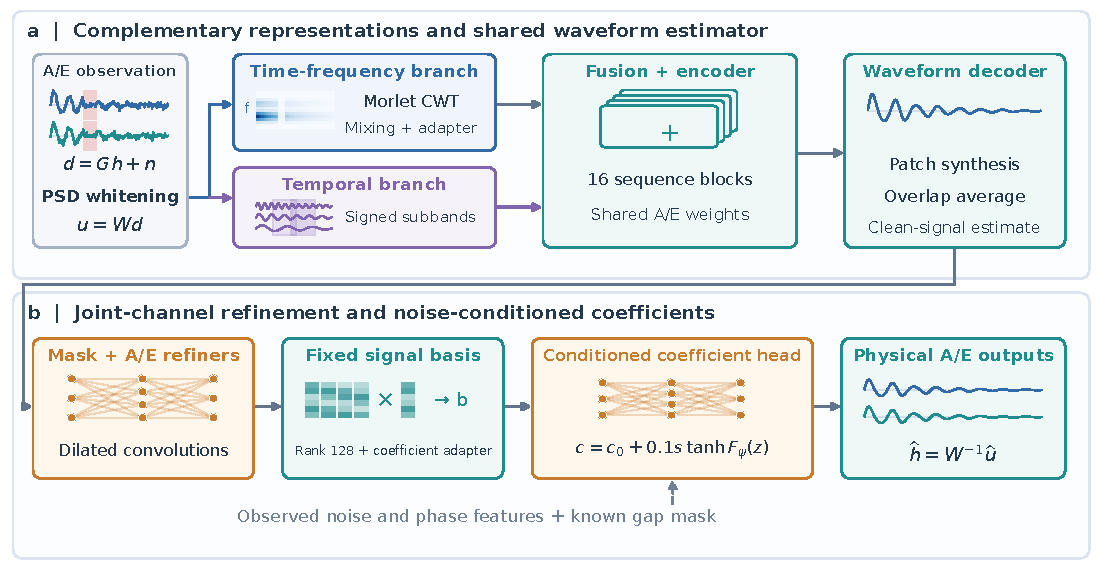
\includegraphics[width=\textwidth]{architecture_dgf_20261015.pdf}
\caption{DGF architecture. The time--frequency and signed temporal representations feed a shared encoder and waveform decoder. Mask-aware and joint-channel refiners precede the signal-basis adapter and conditioned coefficient head. The head adjusts coefficients of a fixed basis; its zero-initialized correction preserves the basis-adapted prediction at initialization. Inverse whitening returns the $A/E$ estimates to physical units. Dashed arrows mark conditioning inputs. The small waveform, transform and network drawings are schematic.}\label{fig:pipeline}\label{fig:architecture}
\end{figure*}

\subsection{Joint-channel refinement and noise-conditioned coefficients}\label{sec:coefficients}
A channel-wise mask-aware residual module receives the observation, intermediate prediction, mask and normalized time coordinate. Its six dilated Conv1d blocks have width 24, kernel size 7 and dilations $1,2,4,8,16,32$, with group normalization and GELU. A second width-32 residual module couples the $A$ and $E$ predictions using the same dilation schedule.

We construct a joint basis $B\in\mathbb R^{2N\times128}$ from the 60,000 clean training waveforms in whitened coordinates. After removing DC and Nyquist, each waveform is normalized to give equal weight to each source. The leading eigenvectors of the resulting second-moment matrix form the basis. Writing $v$ for the refined waveform, the coefficient adapter produces
\begin{align}
\beta&=B^{\mathsf T}P_0v+0.2s\,g_\varphi(z_v),\nonumber\\
b&=B\beta+(I-P_0)v.\label{eq:basis_adapter}
\end{align}
Here $P_0$ removes DC and Nyquist, $s=\max[\operatorname{RMS}(u),10^{-4}]\sqrt{2N}$, and $g_\varphi$ is a $262\to128\to128\to128$ MLP with GELU after the first two linear layers. The vector $z_v$ contains observation, prediction and mask coordinates defined in Appendix~\ref{app:model_analysis}. Since $P_0B=B$, the interior-frequency component $P_0b$ lies in the span of $B$.

The coefficient head predicts the waveform coordinates through
\begin{align}
c_0&=B^{\mathsf T}P_0b,\qquad
c=c_0+0.1s\tanh F_\psi(z),\label{eq:refinement}\\
\widehat u&=Bc+(I-P_0)b,\qquad
\widehat h=W^{-1}\widehat u.\nonumber
\end{align}
Equation~\eqref{eq:refinement} preserves the endpoint components of $b$. At initialization, the final layer gives $F_\psi=0$ and $c=c_0$. Together with $B^{\mathsf T}B=I$ and $P_0b\in\operatorname{span}(B)$, this yields $\widehat u=b$ to floating-point precision.

The 470-dimensional input $z$ contains 262 normalized coefficient and mask coordinates, 16 noise-level and spectral features, and 192 pooled phase features. Appendix~\ref{app:model_analysis} defines each component and its normalization. For the physical-frequency CWT, we use an amplitude-weighted circular phase representation,
\begin{equation}
a_C\{1,\cos\theta_C,\sin\theta_C\},\quad
a_C=\log(1+|C|),\quad\theta_C=\arg C.\label{eq:continuous_phase}
\end{equation}
Amplitude weighting makes the phase features approach zero as the local CWT amplitude approaches zero. Pooling these features to a $4\times8$ grid in each channel gives 192 entries. The head maps 470 inputs to width 192, applies two residual multilayer perceptron (MLP) blocks and outputs 128 coefficients. Each residual block uses layer normalization, two linear layers, GELU and dropout 0.05, and adds 0.25 times its output to the incoming features. The coefficient head has 264,128 parameters. The complete stored model has 9,589,685 parameters.

The head uses the observation, current prediction, mask and noise calibration. Source parameters and clean targets enter simulation, supervision and evaluation.

\subsection{Training objective and data partition}\label{loss}
We define the direct joint-channel inner product by
\begin{equation}
(a|b)_S=4\Delta f\operatorname{Re}
\sum_{c\in\{A,E\}}\sum_{k=1}^{N/2-1}
\frac{\widetilde a_{c,k}\widetilde b_{c,k}^{*}}{S_{c,\rm cal}(f_k)},\label{eq:joint_inner}
\end{equation}
where $\widetilde a=\Delta t\,\operatorname{rfft}(a)$, $\Delta t=1/f_s$ and $\Delta f=f_s/N$. We define the joint-channel mismatch and PSD-weighted network signal-to-noise ratio (SNR) as
\begin{equation}
\mathcal M_{AE}=1-\frac{(h|\widehat h)_S}{\sqrt{(h|h)_S(\widehat h|\widehat h)_S}},\quad
\rho^2=(h|h)_S.\label{eq:joint_mismatch}
\end{equation}
The SNR refers to the complete clean target before signal suppression. We evaluate overlap at the original time and phase. For nonzero waveforms, $\mathcal M_{AE}\in[0,2]$, with values above one for anticorrelated predictions. An overall positive rescaling of the PSD cancels in the normalized overlap; its frequency dependence sets the relative bin weights.

Final two-channel optimization uses
\begin{equation}
\mathcal L=\mathcal M_{AE}+0.2E_S+0.02E_{\rm time,gap},\label{eq:loss}
\end{equation}
with
\begin{align}
E_S&=\frac{(\widehat h-h|\widehat h-h)_S}{(h|h)_S},\nonumber\\
E_{\rm time,gap}&=\frac{\sum_{c,j}(1+2m_j)(\widehat h_{c,j}-h_{c,j})^2}{\sum_{c,j}h_{c,j}^2}.\label{eq:auxiliary_errors}
\end{align}
The objective combines mismatch, normalized noise-weighted waveform error and normalized time-domain waveform error, with a factor-three weight inside the gap. Losses and population mismatches are arithmetic means over sources.

Figure~\ref{fig:training_workflow} summarizes training. The 60,000 physical training sources each contribute three views. Two have independently sampled variable gap widths around the same reference center; the first retains the original noise realization and the second uses independent noise. The third has a 33-s gap and another independent noise realization. The second and third views receive a common input--target sign drawn with equal probability from $\{-1,1\}$ for each source. Widths, noise and signs are drawn once and held fixed across epochs. CWT and db4 features are recomputed from each observation. One epoch contains 180,000 observations.

The validation set contains 1,500 independent sources. Model selection uses the mean direct mismatch over this complete set with uniformly sampled variable gap widths. Fixed 33- and 50-s gaps provide additional checks on the same sources. The independent test set contains 6,000 sources generated after model selection. Population summaries include all generated sources; SNR-conditioned summaries state the corresponding sample counts.

\begin{figure*}[t]
\centering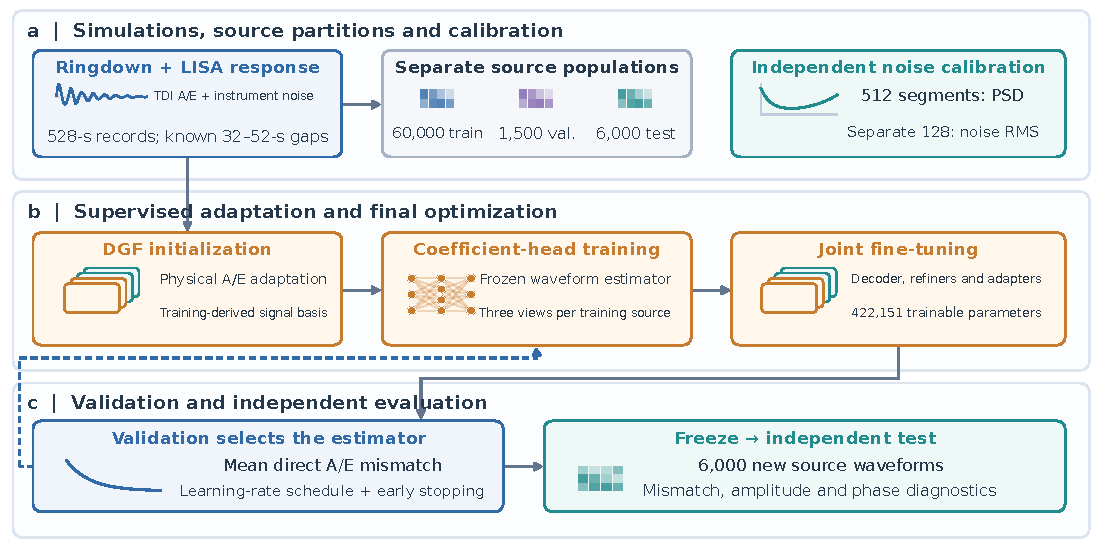
\includegraphics[width=\textwidth]{training_workflow_dgf_20261015.pdf}
\caption{Simulation and training workflow. Physical source populations and noise-calibration realizations are separate. Supervised A/E adaptation initializes the waveform estimator and coefficient adapter; head training and joint fine-tuning then use the augmented training views. Validation controls learning rates, early stopping and model selection. The selected estimator is evaluated on newly generated test sources. Dashed arrows show validation feedback; the small drawings are schematic.}\label{fig:training_workflow}
\end{figure*}

\subsection{Training protocol}\label{sec:training}
We initialize the encoder and waveform synthesis modules from a DGF model adapted to the physical $A/E$ training sources. Appendix~\ref{app:initialization} describes the initialization stages and their objectives. Before full coefficient-head training, we compare phase-only, noise-only and combined feature sets on the first 6,000 training sources. All three heads receive the same 262 coefficient and mask coordinates; the phase-only and noise-only variants set the other feature group to zero. The full 1,500-source validation mean selects the combined head. The selected feature set then undergoes two optimization stages. First, the coefficient head is trained with the waveform estimator held fixed, using cached predictions and features. AdamW uses batches of 1024, weight decay $3\times10^{-4}$ and a five-epoch warmup to learning rate $3\times10^{-4}$. Validation plateaus halve the learning rate. Training has a maximum of 600 epochs, minimum 100, patience 100 and improvement threshold $10^{-6}$.

The second stage jointly trains the decoder, physical-frequency adapter, channel-wise and joint residual modules, coefficient adapter and head. The encoder, transforms and signal basis remain fixed. This stage has 422,151 trainable parameters. Group learning rates range from $5\times10^{-7}$ for the decoder to $10^{-4}$ for the head. It uses batches of 128, the same weight decay, a maximum of 200 epochs, minimum 40 and patience 50. Validation plateaus trigger further learning-rate reductions.

Raw and exponential-moving-average weights, with decay factor 0.995, are evaluated using the complete validation mean. Model selection, early stopping and learning-rate scheduling use validation sources. The independent test set is reserved for the selected estimator. Appendix~\ref{app:model_analysis} gives the numerical conventions, and Appendix~\ref{app:fixed_gaps} reports supplementary evaluation on the same independent test sources.

\section{Reconstruction results}\label{sec:results}
We evaluate the validation-selected checkpoint on 6,000 independent LISA test sources. Each 528-s record contains 1056 samples at 2 Hz and one 32--52-s gap drawn as specified in Sec.~\ref{sec:gaps}. We first report the $\rho\ge10$ population, which contains 5814 sources, together with statistics for the full test set. The distributions include all 6,000 sources. The fixed-duration tests in Appendix~\ref{app:fixed_gaps} use the same source waveforms and noise realizations.

\subsection{Waveform mismatch}\label{subsec:Mismatch}
We evaluate the noise-weighted mismatch in Eq.~\eqref{eq:joint_mismatch} jointly over the $A/E$ channels at the injected time and phase. The corresponding time-domain mismatch is
\begin{equation}
\mathcal M_t=1-\frac{\sum_{c,j}h_{c,j}\widehat h_{c,j}}{\sqrt{\sum_{c,j}h_{c,j}^2\sum_{c,j}\widehat h_{c,j}^2}}.
\end{equation}
These normalized overlaps measure waveform agreement. Population means assign equal weight to each source. We report amplitude-sensitive residuals separately in Sec.~\ref{subsec:MeanSquaredError}.

\begin{table*}[t]\centering
\caption{DGF reconstruction accuracy for the independent variable-gap test. The first row gives the 5814 sources with network SNR $\rho\ge10$; the second includes all 6,000 test sources. The overlap is evaluated at the injected time and phase.}\label{tab:results}
\begin{tabular}{lrrrrr}\hline\hline
Population & $n$ & Mean $\mathcal M_{AE}$ & Median $\mathcal M_{AE}$ & 95th percentile $\mathcal M_{AE}$ & Mean $\mathcal M_t$\\\hline
$\rho\ge10$ & 5814 & 0.00532 & 0.00241 & 0.01970 & 0.00934 \\
All test signals & 6000 & 0.00852 & 0.00254 & 0.02782 & 0.01367 \\
\hline\hline\end{tabular}\end{table*}

For $\rho\ge10$, DGF achieves a mean direct noise-weighted mismatch of 0.00532, a median of 0.00241 and a 95th percentile of 0.01970 (Table~\ref{tab:results}). These values quantify recovery at the original arrival time and phase. The full 6,000-source population has mean 0.00852, median 0.00254 and 95th percentile 0.02782. Figure~\ref{fig:mismatch} shows its complete mismatch distributions. Network SNR spans 1.69--923.52, with median 54.77; Fig.~\ref{fig:snr_gap} shows the dependence on SNR and gap location. A regularized fit in the same training-derived signal basis has mean mismatch 0.04131 for $\rho\ge10$, compared with 0.00532 for DGF on identical observations. Appendix~\ref{app:basis_comparison} specifies this fit and quantifies basis representation error.
\begin{figure*}[t]\centering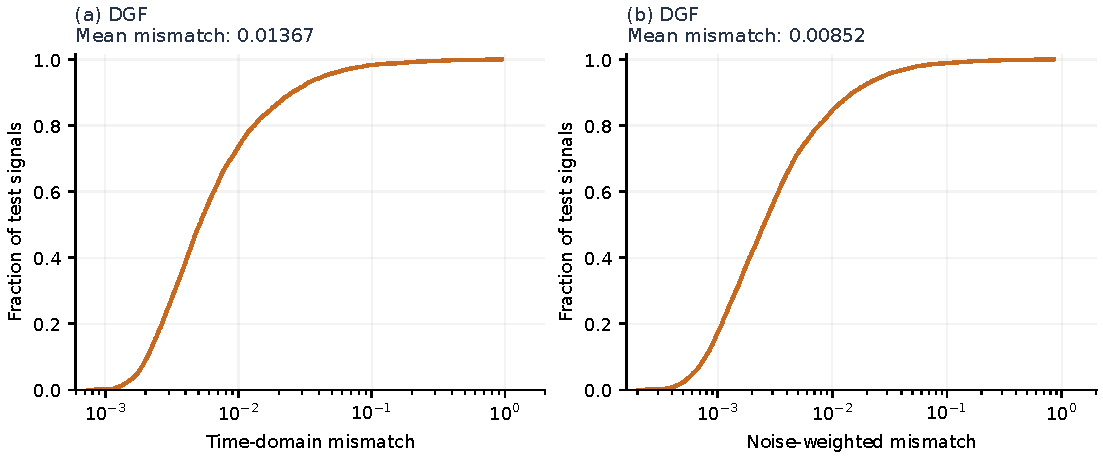
\includegraphics[width=\textwidth]{latest_mismatch.pdf}
\caption{Empirical cumulative distribution functions of time-domain and noise-weighted mismatch for the complete test population. The logarithmic axes show the full range of reconstruction errors.}\label{fig:mismatch}\end{figure*}

\subsection{Gap location and waveform recovery}
We characterize gap location using the peak of the joint analytic envelope $[\sum_c|h_c+i\mathcal H[h_c]|^2]^{1/2}$, where $\mathcal H$ denotes the Hilbert transform. In the full test population, the peak lies inside the gap for 1935 sources. Their mean noise-weighted mismatch is 0.00912, with median 0.00285. For the remaining 4065 sources, the mean is 0.00823. These statistics reflect the joint distributions of gap location, source parameters and noise realizations within each group.

\begin{figure*}[t]\centering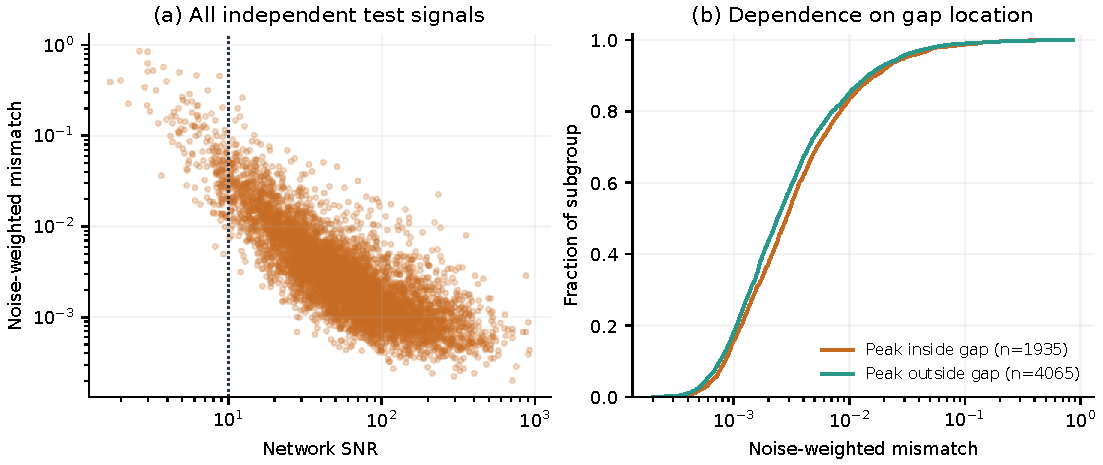
\includegraphics[width=\textwidth]{latest_snr_gap.pdf}
\caption{Dependence of reconstruction accuracy on network SNR and gap location for the independent test population. (a) Joint noise-weighted mismatch versus network SNR, with the dotted line at $\rho=10$. (b) Conditional mismatch distributions according to whether the joint signal-envelope peak falls inside the gap. The two groups partition the test population.}\label{fig:snr_gap}\end{figure*}



We also characterize gap severity by $\eta=\sum_{c,j}m_jh_{c,j}^2/\sum_{c,j}h_{c,j}^2$ and $T_{\rm gap}/\tau_{220}$. In the $\rho\ge10$ population, their medians are 0.289 and 0.238, and their 95th percentiles are 0.666 and 1.44. The 2638 sources with $\eta<0.25$ have mean mismatch 0.00469; the 127 with $\eta\ge0.75$ have mean 0.01583. These conditional summaries include variation in source parameters, noise and gap duration.

Figure~\ref{fig:examples} shows two $\rho\ge10$ sources reconstructed across 36- and 45-s gaps, with noise-weighted mismatches $5.59\times10^{-4}$ and $6.07\times10^{-4}$. The gaps contain 42.7\% and 56.8\% of the respective joint signal squared norms. Their gap-local relative errors are 4.6\% and 3.7\%, and both channels retain the decaying oscillations through the missing intervals. For these two sources, the windows extend for approximately 4.9 dominant-mode damping times after the response peak.
\begin{figure*}[tp]\centering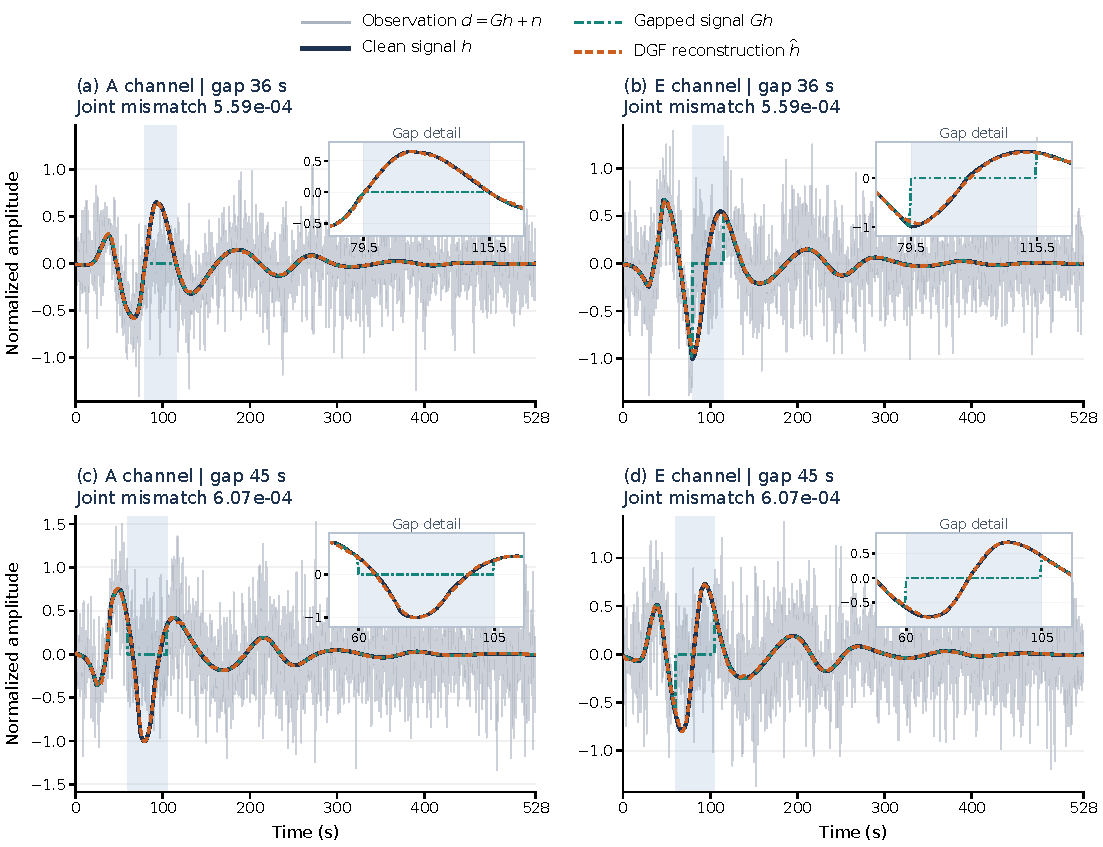
\includegraphics[width=0.885\textwidth]{latest_examples.pdf}
\caption{Waveform reconstruction for two $\rho\ge10$ sources across 36- and 45-s gaps in the $A$ (left) and $E$ (right) channels. Each panel superposes the noisy observation $d=Gh+n$ (gray), clean signal $h$, gapped clean signal $Gh$ and DGF reconstruction $\widehat h$ over the full 528-s record; insets resolve the gap. Shading marks signal suppression, with noise retained. For each source, all curves in both channels are divided by $H_{\rm TDI}=\max_{c,j}|h_{c,j}|$ and connect the original 0.5-s samples. Source seeds, from top to bottom, are 2038202231 and 2038201952. The example criteria are given in Appendix~\ref{app:model_analysis}.}\label{fig:examples}\par\vspace{8pt}
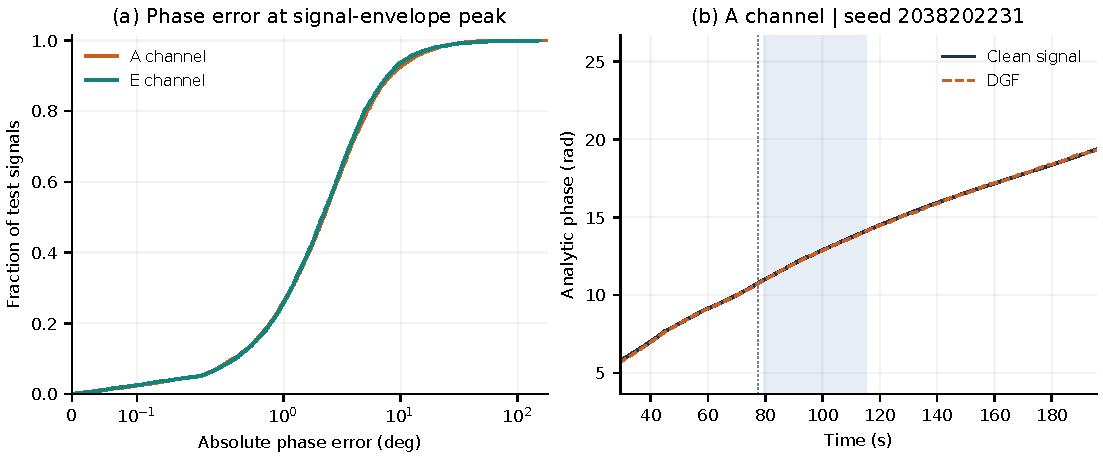
\includegraphics[width=0.885\textwidth]{latest_phase.pdf}
\caption{(a) Absolute phase-error distributions for all 6,000 sources in each channel. (b) Analytic phase of the $A$ channel for source 2038202231, also shown in Fig.~\ref{fig:examples}(a). The displayed clean-signal envelope exceeds 10\% of its peak. The clean phase is $\phi_c=\operatorname{unwrap}(\arg z_c)$; the displayed reconstruction is $\phi_c+\arg(\widehat z_cz_c^*)$. Unwrapping removes adjacent jumps greater than $\pi$. Shading marks the gap and the dotted line marks the clean envelope peak.}\label{fig:phase}\end{figure*}

\subsection{Phase recovery}\label{subsec:PhaseRecoveryAlignment}
For each channel, define $z_c=h_c+i\mathcal H[h_c]$ and $\widehat z_c=\widehat h_c+i\mathcal H[\widehat h_c]$. At the clean-signal envelope peak $j_{\star,c}$, the phase error is
\begin{equation}
\Delta\phi_c=\arg[\widehat z_{c,j_{\star,c}}z_{c,j_{\star,c}}^*].
\end{equation}
For the complete test population, the mean absolute phase errors are $3.84^\circ$ in $A$ and $3.79^\circ$ in $E$. The corresponding medians are $2.19^\circ$ and $2.14^\circ$, and the 95th percentiles are $12.72^\circ$ and $11.58^\circ$. These statistics describe the analytic phase of each channel at its clean-signal envelope peak. Figure~\ref{fig:phase}(b) compares analytic phases for the $A$ channel of one example. Individual quasinormal-mode phases require a separate mode decomposition.

To measure recovery within the interval, we define the envelope-weighted gap phase error
\begin{equation}
\Phi_{\rm gap}=\left[\frac{\sum_{c,j}m_j|z_{c,j}|^2[\arg(\widehat z_{c,j}z_{c,j}^*)]^2}{\sum_{c,j}m_j|z_{c,j}|^2}\right]^{1/2}.\label{eq:gap_phase}
\end{equation}
Among the 1885 sources with $\rho\ge10$ and the joint envelope peak inside the gap, its mean, median and 95th percentile are $4.92^\circ$, $3.89^\circ$ and $11.61^\circ$. Over the complete peak-inside-gap population of 1935 sources, the corresponding mean is $5.51^\circ$.



\subsection{Amplitude and spectral fidelity}\label{subsec:MeanSquaredError}\label{subsec:AmplitudeDensityFrequencySpectrum}
Normalized overlap is invariant under positive amplitude rescaling. We therefore evaluate the relative waveform error
\begin{equation}
E=\frac{\left[\sum_{c,j}(\widehat h_{c,j}-h_{c,j})^2\right]^{1/2}}{\left[\sum_{c,j}h_{c,j}^2\right]^{1/2}}.
\end{equation}
For the complete test population, $E$ has mean 0.13424, median 0.10337 and 95th percentile 0.30008. The mean signed norm bias, $\|\widehat h\|_2/\|h\|_2-1$, is -0.01301. The norm bias measures the fractional difference between reconstructed and target waveform norms; $E$ measures their full waveform difference.

For the 1935 sources with envelope peaks inside the gap, the gap-local relative error $\|m(\widehat h-h)\|_2/\|mh\|_2$ has mean 0.13552 and median 0.10337. The denominator is the Euclidean norm of the clean waveform restricted to the gap. The full-waveform error $E$ remains the common amplitude-sensitive measure for all sources.

Figure~\ref{fig:tdi_log_amplitudes} plots waveform absolute values for the sources in Fig.~\ref{fig:examples}. In these two examples, the logarithmic scale reveals differences in the late-time waveform and near zero crossings. Figure~\ref{fig:psd} compares population-averaged target, residual and instrument-noise spectra. For $\rho\ge10$, the mean normalized noise-weighted squared waveform error $E_S$ is 0.01190; its complete-population mean is 0.01786. The periodogram definition is given in Appendix~\ref{app:model_analysis}.
\begin{figure*}[tp]\centering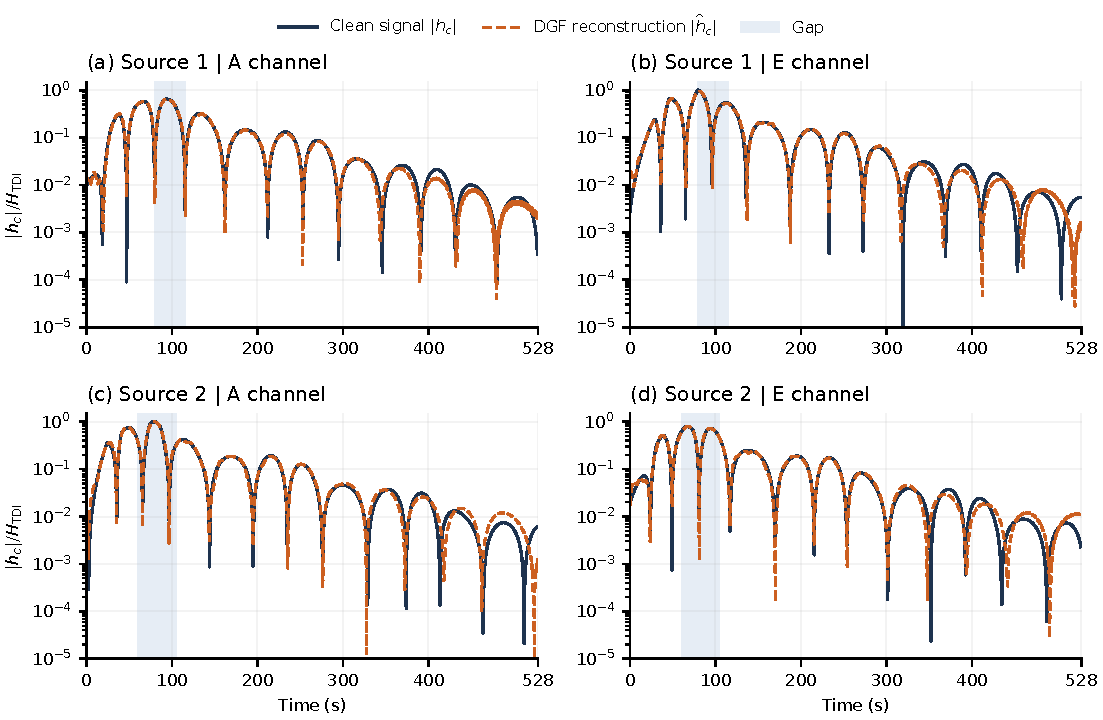
\includegraphics[width=\textwidth]{tdi_log_amplitudes_20261015.pdf}
\caption{Absolute values of the clean and reconstructed $A$ (left) and $E$ (right) waveforms for the sources in Fig.~\ref{fig:examples}. Each row uses the common scale $H_{\rm TDI}=\max_{c,j}|h_{c,j}|$ from the clean signal. Shading marks the gap. The logarithmic axis resolves small-amplitude structure and differences near zero crossings. The curves connect the native samples used in Fig.~\ref{fig:examples}.}\label{fig:tdi_log_amplitudes}
\par\vspace{8pt}
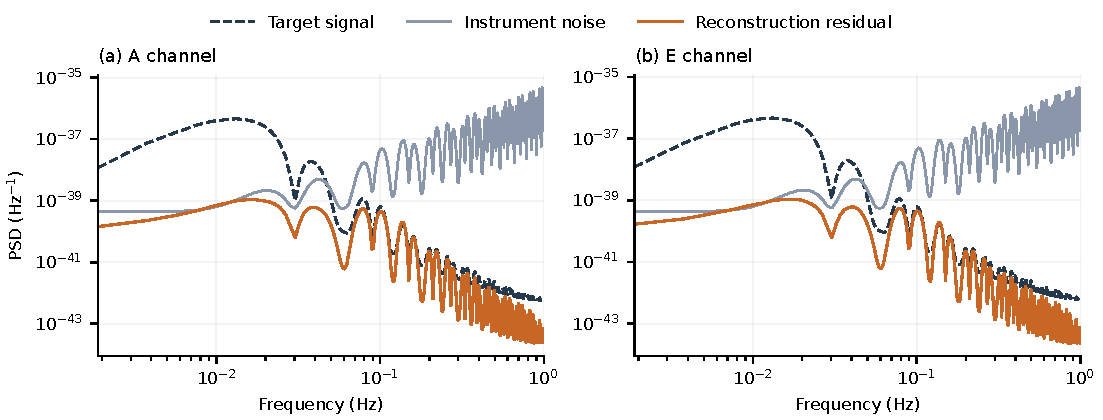
\includegraphics[width=\textwidth]{latest_residual_psd.pdf}
\caption{Mean power spectral densities of the target signal $h$, reconstruction residual $\widehat h-h$ and instrument noise in the $A/E$ channels over all test sources. Each periodogram uses a rectangular window, constant detrending and one-sided density normalization, followed by an arithmetic mean over sources. Only interior Fourier bins are shown. Fractional-frequency PSDs have units $\mathrm{Hz}^{-1}$.}\label{fig:psd}\end{figure*}




\section{Discussion and Conclusions}\label{sec:discussion}
DGF reconstructs black hole ringdown waveforms by combining time--frequency information with signed multiscale temporal features. A shared encoder and joint-channel refinement estimate the clean LISA $A/E$ waveforms from the noisy observation and gap mask. For the 5814 test sources with $\rho\ge10$ and 32--52-s gaps, the mean direct noise-weighted mismatch is 0.00532. The mean over all 6,000 independent sources is 0.00852. The waveform comparisons show recovery of the decaying oscillations across intervals containing the signal peak, while amplitude residuals complement the normalized overlap.

For the full test population, the mean absolute analytic-phase errors at the envelope peak are $3.84^\circ$ and $3.79^\circ$ in $A$ and $E$. The two waveform examples show visible late-time differences on a logarithmic scale. Their contribution to a full-record error depends on its weighting. Assessing individual mode frequencies, damping times and phases requires mode-resolved fits over specified time intervals. The fixed-duration tests and signal-basis comparison complement the variable-gap results. The latter separates linear fitting in the learned subspace from DGF coefficient prediction.

The simulations cover nonspinning progenitor binaries, an idealized equal-arm constellation and stationary Gaussian instrument noise. They assume an event-centered window, one known gap and the signal history specified in Sec.~\ref{sec:physical_signals}. Tests with continuous merger histories would assess sensitivity to the pre-reference ring-up entering the TDI delays. Tests with moving unequal-arm constellations and nonstationary noise would assess sensitivity to response and noise-model errors. Independently perturbed mode amplitudes, phases and frequencies would test how much structure outside the training relations is preserved.

DGF provides a clean-waveform point estimate for inspecting ringdown structure and initializing waveform fits. A subsequent parameter analysis under Eq.~\eqref{eq:observation} would use a likelihood constructed from $d-Gh(\theta)$ and the noise covariance. Posterior-bias and coverage tests remain part of that analysis. Previous LISA gap studies~\cite{Baghi2019,Mao:2025cae} motivate this validation alongside waveform-level metrics. Quantifying reconstruction uncertainty and testing the recovery of individual modes are the next steps toward applications in black hole spectroscopy.

\begin{acknowledgments}
The authors thank He Wang and Yiyang Guo for helpful discussions. This research is supported in part by the National Key R\&D Program of China, grant number 2020YFC2201300, and the National Natural Science Foundation of China, grant numbers 12035016, 12375058 and 12361141825.

\end{acknowledgments}
\clearpage
\appendix
\section{Implementation and reproducibility}\label{app:model_analysis}
\subsection{Representations and attention}
For each $A/E$ channel, the backbone CWT array has shape $2\times16\times264$, and the temporal patches and fused features have shape $8\times32\times64$. For a feature matrix $Z\in\mathbb R^{32\times64}$, attention is computed as
\begin{equation}
A(Z)=\operatorname{softmax}(ZZ^{\mathsf T}/\sqrt{64})Z.
\end{equation}
Each of the eight feature channels applies this operation, followed by feedforward transformations, residual connections and normalization. Attention spans the full sequence.

The eight db4 channels reconstruct $A_8,D_8,D_7,\ldots,D_2$ with zero padding. The decoder combines reconstructed patches by overlap averaging and subband summation. The encoder embedding and decoder patch maps use independent parameter tensors.

\subsection{Numerical and test conventions}
The RMS floor in whitened coordinates is $10^{-4}$ for coefficient and residual normalization. Training spectral target and prediction squared norms are floored at $10^{-12}$ for finite numerical division, and physical-time relative-error denominators use the same floor in the scaled working representation. Physical evaluation uses float64 transforms, the common frozen PSD and the complete target norm. Overlap is clipped to $[-1,1]$ to bound roundoff. A zero prediction is assigned mismatch one; a zero target triggers a dataset validation failure.

Source seeds are consecutive integers starting at 2028000000, 2028100000 and 2038200000 for training, validation and testing, respectively. The selected checkpoint has SHA-256 prefix \texttt{0ffce08b8856}; the reproducibility manifest gives full hashes and separate noise seeds.

The implementation uses PyCBC 2.8.2, LALSuite 7.25.1, \texttt{fastlisaresponse} 1.1.17, LISA Analysis Tools 1.2.8, \texttt{ssqueezepy} 0.6.5 and \texttt{pytorch\_wavelets} 1.3.0. The computational source version is \texttt{ae47cce8a5c0}. Code is maintained at \url{https://github.com/ljq2088/RingdownGapFilling}. Checkpoints, calibration arrays and evaluation records are available from the authors on request; the accompanying reproducibility manifest identifies the assets and software versions.

Figure~\ref{fig:examples} uses sources with the joint peak in the gap, $\rho\ge10$, at least four $\tau_{220}$ of post-peak coverage and six visible extrema per channel. Full-record and gap-local errors are below 6\%, and peak-phase errors below $2.5^\circ$. The plotting manifest gives the channel-balance, native-sample curvature and noise-amplitude criteria.

Each channel-specific phase distribution contains one value per test source. Gap-local errors use the target norm within the gap; the peak-inside-gap population provides intervals containing appreciable signal.



\subsection{Coefficient-head inputs}
For an intermediate prediction $y\in\{v,b\}$, let $a_y=B^{\mathsf T}P_0y$, $q=B^{\mathsf T}u$, $r=\operatorname{RMS}(u)$ over both channels and $s=\max(r,10^{-4})\sqrt{2N}$. Write $R_c(x)=\operatorname{RMS}(P_0x_c)$ and $\nu_c$ for the calibrated whitened-noise RMS. The coefficient adapter uses the 262-dimensional coordinates for $y=v$; the final head uses those for $y=b$ and adds noise and phase features. Table~\ref{tab:head_features} lists the components. Before computing noise features, $R_c(u)$ and $\nu_c$ are floored at $10^{-6}$. Log ratios are clipped to $[-8,8]$ and logarithms of the form $\log(1+x)$ to a maximum of 8.

\begin{table*}[t]\centering
\caption{Input features of the conditioned coefficient head. The first group also supplies the coefficient adapter. $a$ and $L$ denote the local gap start and length. The phase features use the physical-frequency CWT.}\label{tab:head_features}
\begin{tabular}{lrl}\hline\hline
Group & Dimension & Components\\\hline
Prediction coefficients & 128 & $a_b/s$\\
Observation coefficients & 128 & $q/s$\\
Gap coordinates & 3 & $a/N$, $(a+L)/N$, $L/N$\\
Channel RMS ratios & 2 & $\operatorname{RMS}(u_c)/\max(r,10^{-4})$\\
Coefficient norm & 1 & $\|a_b\|_2/s$\\\hline
Noise-level ratios & 4 & $\log[R_c(u)/\nu_c]$, $\log[1+\nu_c/R_c(u)]$, for each channel\\
Frequency-band ratios & 8 & $[2\sum_{k\in K}|\operatorname{rfft}(u_c)_k|^2/N^2]^{1/2}/R_c(u)$\\
Residual and predicted RMS & 4 & $\log[1+R_c(u-b)/\nu_c]$, $\log[1+R_c(b)/\nu_c]$\\\hline
Pooled phase representation & 192 & $\log(1+|C|)\{1,\cos\theta_C,\sin\theta_C\}$; $4\times8$ pooling per channel\\
\hline\hline\end{tabular}

\smallskip\parbox{0.96\textwidth}{The four frequency-bin groups are $K=\{1,\ldots,4\}$, $\{5,\ldots,16\}$, $\{17,\ldots,64\}$ and $\{65,\ldots,527\}$. Both channels contribute to each feature group, giving $262+16+192=470$ inputs.}
\end{table*}

\subsection{Periodograms}
For a series $x_j$, the one-sided periodogram used in Fig.~\ref{fig:psd} is
\begin{equation}
P_x(f_k)=\frac{\kappa_k}{Nf_s}\left|\sum_{j=0}^{N-1}(x_j-\bar x)e^{-2\pi i jk/N}\right|^2,
\end{equation}
with $\kappa_k=2$ at interior bins and 1 at DC and Nyquist. We use a rectangular window and average the individual source periodograms arithmetically. The target, residual and noise series receive identical processing.

\subsection{Initialization and adaptation}\label{app:initialization}
The supplied legacy DGF weights initialize reproduction. Their training code uses pointwise squared and absolute errors on a separate 10,000-waveform simulation bank. Physical $A/E$ adaptation uses 12,000 training sources with 33-s gaps and objective $\mathcal M_{AE}+0.5E_S+0.5E_{\rm time,gap}$, then 60,000 sources for joint-channel and physical-frequency adaptation with an additional Hann-windowed penalty.

The signal basis uses the 60,000 clean training directions. Coefficient-adapter training and variable-gap joint training use $\mathcal M_{AE}+0.5E_S+0.05E_{\rm time,gap}+0.02[\mathcal M_H+0.5(\sqrt{1+E_H}-1)]$, where $\mathcal M_H,E_H$ use a Hann window and its noise calibration. All physical-data stages select on the same complete validation mean. Their configurations and weights are identified in the manifest. The final-head initialization has identifier \texttt{a1e9959a7a95}; final optimization uses Eq.~\eqref{eq:loss} and Sec.~\ref{sec:training}, followed by new independent testing.

\section{Fixed-duration gaps and reference comparison}\label{app:fixed_gaps}
We evaluate 33- and 50-s gaps on the same 6,000 source waveforms and noise realizations, preserving each gap's center. Table~\ref{tab:fixed_gaps} reports both the $\rho\ge10$ and full-population results. For $\rho\ge10$, the mean joint noise-weighted mismatches are 0.00438 and 0.00715 for 33- and 50-s gaps, respectively. These tests vary the mask while holding the physical sources and noise fixed.
\begin{table}[t]\centering\setlength{\tabcolsep}{2pt}
\caption{Additional gap-duration tests on the same independent sources. For each duration, the $\rho\ge10$ row contains 5814 sources and the complete-population row contains all 6,000 sources.}\label{tab:fixed_gaps}
\begin{tabular}{lrrr}\hline\hline
Gap and SNR & Mean $\mathcal M_{AE}$ & Median $\mathcal M_{AE}$ & \shortstack{95th\\percentile}\\\hline
33 s / $\rho\ge10$ & 0.00438 & 0.00195 & 0.01608\\
33 s / all & 0.00716 & 0.00204 & 0.02389\\
50 s / $\rho\ge10$ & 0.00715 & 0.00334 & 0.02498\\
50 s / all & 0.01112 & 0.00350 & 0.03653\\
\hline\hline\end{tabular}\end{table}

A reference DGF configuration with joint-channel synthesis and the training-derived signal basis is evaluated on the identical test observations. This reference uses the variable-gap joint-training checkpoint \texttt{a1e9959a7a95}, comprising the waveform estimator and coefficient adapter. For variable gaps across all 6,000 test sources, its mean mismatch is 0.00868, compared with 0.00852 for the selected model. For each source, define $\Delta\mathcal M=\mathcal M_{\rm DGF}-\mathcal M_{\rm ref}$. Its mean is $-1.61\times10^{-4}$. A paired bootstrap with 5,000 source-level resamples gives the 95\% percentile interval $[-2.45\times10^{-4},-8.11\times10^{-5}]$ for the mean difference. This comparison concerns the complete fitted configurations, including their synthesis parameters and coefficient heads.



\section{Signal-basis fitting and representation error}\label{app:basis_comparison}
We compare DGF with a linear estimator using the same rank-128 basis $B$. Four orthonormal DC and Nyquist directions, collected in $B_{\rm end}$, supply endpoint degrees of freedom. Each clean training waveform is divided by $\|P_0Wh\|_2$ before projecting onto $[B,B_{\rm end}]$. The mean squared coefficients define prior variances, floored at $10^{-16}$. Let $D$ contain their square roots and $Q=[B,B_{\rm end}]D$. The regularized estimate is
\begin{align}
\widehat a_\lambda&=\arg\min_a\{\|P_0W(d-GW^{-1}Qa)\|_2^2+\lambda\|a\|_2^2\},\nonumber\\
\widehat h_{\rm lin}&=W^{-1}Q\widehat a_\lambda.
\end{align}
Thus the forward map applies the same physical signal suppression before whitening. The Gaussian coefficient prior uses training data only. A grid containing zero and $10^{-6},10^{-5},\ldots,10^2$ selects $\lambda=10^{-3}$ by the complete validation mean. Table~\ref{tab:basis_fit} compares this estimator and DGF on identical test observations. The complete-population paired mean difference, DGF minus linear fit, is $-0.04341$, with 95\% percentile bootstrap interval $[-0.04532,-0.04156]$ from 5,000 source-level resamples.

\begin{table}[t]\centering\setlength{\tabcolsep}{3pt}
\caption{Direct noise-weighted mismatch for DGF and the training-prior regularized basis fit.}\label{tab:basis_fit}
\begin{tabular}{llrrr}\hline\hline
Population & Estimator & Mean & Median & 95th perc.\\\hline
$\rho\ge10$ & DGF & 0.00532 & 0.00241 & 0.01970\\
& Basis fit & 0.04131 & 0.02030 & 0.14912\\
All sources & DGF & 0.00852 & 0.00254 & 0.02782\\
& Basis fit & 0.05193 & 0.02141 & 0.21892\\
\hline\hline\end{tabular}\end{table}

To isolate representation error, we project each clean target onto the first $r$ columns of $B$ in whitened coordinates. For $r=32,64,128$, the mean mismatches are 0.03690, 0.00410 and $1.65\times10^{-4}$ over all sources; the corresponding $\rho\ge10$ means are 0.03322, 0.00319 and $1.11\times10^{-4}$. This target projection measures the subspace approximation error.


\clearpage
\bibliography{DGF_references}
\end{document}
